\documentclass{standalone}
\usepackage{tikz}
\usetikzlibrary{patterns, positioning}

\begin{document}
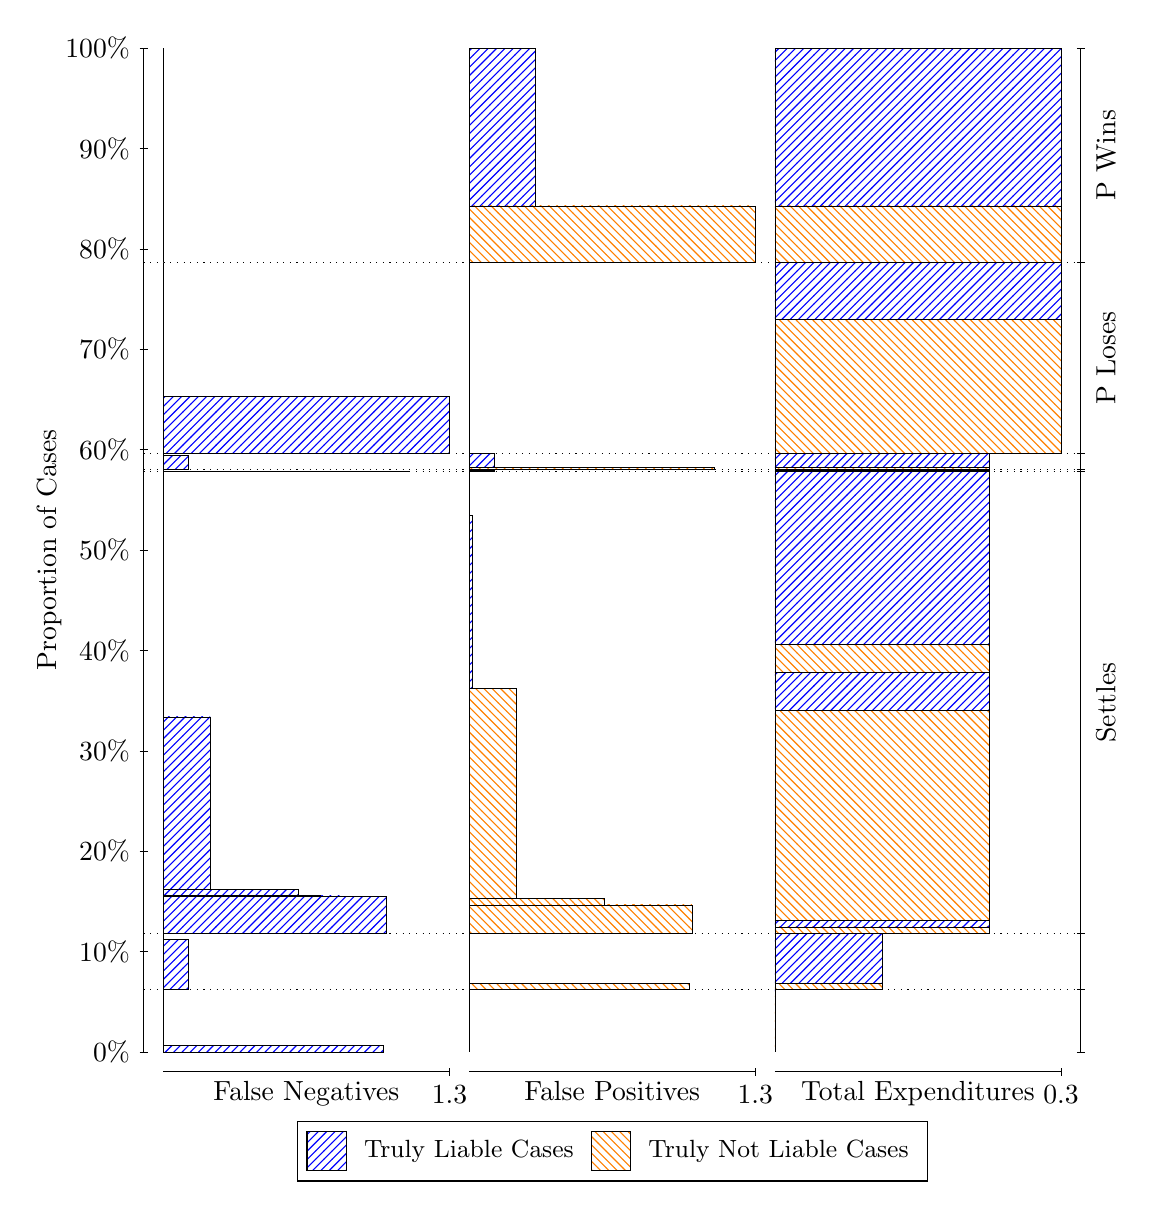
\begin{tikzpicture}
\draw[black, very thin] (1.5,1.75) -- (1.5,14.5);
\node[rotate=90, anchor=center] at (0.3, 8.125) {Proportion of Cases};
\draw[black, very thin] (1.45,1.75) -- (1.55,1.75);
\node[anchor=east] at (1.45, 1.75) {0\%};
\draw[black, very thin] (1.45,3.025) -- (1.55,3.025);
\node[anchor=east] at (1.45, 3.025) {10\%};
\draw[black, very thin] (1.45,4.3) -- (1.55,4.3);
\node[anchor=east] at (1.45, 4.3) {20\%};
\draw[black, very thin] (1.45,5.575) -- (1.55,5.575);
\node[anchor=east] at (1.45, 5.575) {30\%};
\draw[black, very thin] (1.45,6.85) -- (1.55,6.85);
\node[anchor=east] at (1.45, 6.85) {40\%};
\draw[black, very thin] (1.45,8.125) -- (1.55,8.125);
\node[anchor=east] at (1.45, 8.125) {50\%};
\draw[black, very thin] (1.45,9.4) -- (1.55,9.4);
\node[anchor=east] at (1.45, 9.4) {60\%};
\draw[black, very thin] (1.45,10.675) -- (1.55,10.675);
\node[anchor=east] at (1.45, 10.675) {70\%};
\draw[black, very thin] (1.45,11.95) -- (1.55,11.95);
\node[anchor=east] at (1.45, 11.95) {80\%};
\draw[black, very thin] (1.45,13.225) -- (1.55,13.225);
\node[anchor=east] at (1.45, 13.225) {90\%};
\draw[black, very thin] (1.45,14.5) -- (1.55,14.5);
\node[anchor=east] at (1.45, 14.5) {100\%};

\draw[black, very thin] (13.4,1.75) -- (13.4,14.5);
\draw[black, very thin] (13.35,1.75) -- (13.45,1.75);
\node[anchor=west] at (13.35, 1.75) {};
\draw[black, very thin] (13.35,2.5474) -- (13.45,2.5474);
\node[anchor=west] at (13.35, 2.5474) {};
\draw[black, very thin] (13.35,3.258) -- (13.45,3.258);
\node[anchor=west] at (13.35, 3.258) {};
\draw[black, very thin] (13.35,9.1186) -- (13.45,9.1186);
\node[anchor=west] at (13.35, 9.1186) {};
\draw[black, very thin] (13.35,9.1492) -- (13.45,9.1492);
\node[anchor=west] at (13.35, 9.1492) {};
\draw[black, very thin] (13.35,9.3549) -- (13.45,9.3549);
\node[anchor=west] at (13.35, 9.3549) {};
\draw[black, very thin] (13.35,11.775) -- (13.45,11.775);
\node[anchor=west] at (13.35, 11.775) {};
\draw[black, very thin] (13.35,14.5) -- (13.45,14.5);
\node[anchor=west] at (13.35, 14.5) {};

\draw[black, very thin, pattern color=blue, pattern=north east lines] (1.75,1.75) rectangle (4.5449,1.8339);
\draw[black, very thin, pattern color=orange, pattern=north west lines] (1.75,1.8339) rectangle (1.75,2.5474);
\draw[black, very thin, pattern color=blue, pattern=north east lines] (1.75,2.5474) rectangle (2.0644,3.1839);
\draw[black, very thin, pattern color=orange, pattern=north west lines] (1.75,3.1839) rectangle (1.75,3.258);
\draw[black, very thin, pattern color=blue, pattern=north east lines] (1.75,3.258) rectangle (4.5798,3.7276);
\draw[black, very thin, pattern color=blue, pattern=north east lines] (1.75,3.7276) rectangle (4.3003,3.7297);
\draw[black, very thin, pattern color=blue, pattern=north east lines] (1.75,3.7297) rectangle (4.0208,3.7319);
\draw[black, very thin, pattern color=blue, pattern=north east lines] (1.75,3.7319) rectangle (3.7413,3.7341);
\draw[black, very thin, pattern color=blue, pattern=north east lines] (1.75,3.7341) rectangle (3.7413,3.7341);
\draw[black, very thin, pattern color=blue, pattern=north east lines] (1.75,3.7341) rectangle (3.4619,3.8146);
\draw[black, very thin, pattern color=blue, pattern=north east lines] (1.75,3.8146) rectangle (3.1824,3.8149);
\draw[black, very thin, pattern color=blue, pattern=north east lines] (1.75,3.8149) rectangle (2.9029,3.8153);
\draw[black, very thin, pattern color=blue, pattern=north east lines] (1.75,3.8153) rectangle (2.6234,3.8156);
\draw[black, very thin, pattern color=blue, pattern=north east lines] (1.75,3.8156) rectangle (2.3439,6.006);
\draw[black, very thin, pattern color=orange, pattern=north west lines] (1.75,6.006) rectangle (1.75,9.1186);
\draw[black, very thin, pattern color=blue, pattern=north east lines] (1.75,9.1186) rectangle (4.8593,9.1247);
\draw[black, very thin, pattern color=orange, pattern=north west lines] (1.75,9.1247) rectangle (1.75,9.1492);
\draw[black, very thin, pattern color=blue, pattern=north east lines] (1.75,9.1492) rectangle (2.0644,9.3263);
\draw[black, very thin, pattern color=orange, pattern=north west lines] (1.75,9.3263) rectangle (1.75,9.3549);
\draw[black, very thin, pattern color=blue, pattern=north east lines] (1.75,9.3549) rectangle (5.3833,10.073);
\draw[black, very thin, pattern color=orange, pattern=north west lines] (1.75,10.073) rectangle (1.75,11.775);
\draw[black, very thin, pattern color=orange, pattern=north west lines] (1.75,11.775) rectangle (1.75,12.495);
\draw[black, very thin, pattern color=blue, pattern=north east lines] (1.75,12.495) rectangle (1.75,14.5);
\draw[black, very thin, pattern color=orange, pattern=north west lines] (5.6333,1.75) rectangle (5.6333,2.4635);
\draw[black, very thin, pattern color=blue, pattern=north east lines] (5.6333,2.4635) rectangle (5.6333,2.5474);
\draw[black, very thin, pattern color=orange, pattern=north west lines] (5.6333,2.5474) rectangle (8.4282,2.6214);
\draw[black, very thin, pattern color=blue, pattern=north east lines] (5.6333,2.6214) rectangle (5.6333,3.258);
\draw[black, very thin, pattern color=orange, pattern=north west lines] (5.6333,3.258) rectangle (8.4631,3.6174);
\draw[black, very thin, pattern color=orange, pattern=north west lines] (5.6333,3.6174) rectangle (8.1837,3.6176);
\draw[black, very thin, pattern color=orange, pattern=north west lines] (5.6333,3.6176) rectangle (7.9042,3.6179);
\draw[black, very thin, pattern color=orange, pattern=north west lines] (5.6333,3.6179) rectangle (7.6247,3.6182);
\draw[black, very thin, pattern color=orange, pattern=north west lines] (5.6333,3.6182) rectangle (7.3452,3.6961);
\draw[black, very thin, pattern color=orange, pattern=north west lines] (5.6333,3.6961) rectangle (7.0657,3.698);
\draw[black, very thin, pattern color=orange, pattern=north west lines] (5.6333,3.698) rectangle (6.7862,3.6998);
\draw[black, very thin, pattern color=orange, pattern=north west lines] (5.6333,3.6998) rectangle (6.5067,3.7016);
\draw[black, very thin, pattern color=orange, pattern=north west lines] (5.6333,3.7016) rectangle (6.2272,6.3705);
\draw[black, very thin, pattern color=blue, pattern=north east lines] (5.6333,6.3705) rectangle (5.6683,8.561);
\draw[black, very thin, pattern color=blue, pattern=north east lines] (5.6333,8.561) rectangle (5.6333,9.1186);
\draw[black, very thin, pattern color=orange, pattern=north west lines] (5.6333,9.1186) rectangle (5.9478,9.1431);
\draw[black, very thin, pattern color=blue, pattern=north east lines] (5.6333,9.1431) rectangle (5.6333,9.1492);
\draw[black, very thin, pattern color=orange, pattern=north west lines] (5.6333,9.1492) rectangle (8.7426,9.1778);
\draw[black, very thin, pattern color=blue, pattern=north east lines] (5.6333,9.1778) rectangle (5.9478,9.3549);
\draw[black, very thin, pattern color=orange, pattern=north west lines] (5.6333,9.3549) rectangle (5.6333,11.057);
\draw[black, very thin, pattern color=blue, pattern=north east lines] (5.6333,11.057) rectangle (5.6333,11.775);
\draw[black, very thin, pattern color=orange, pattern=north west lines] (5.6333,11.775) rectangle (9.2667,12.495);
\draw[black, very thin, pattern color=blue, pattern=north east lines] (5.6333,12.495) rectangle (6.4718,14.5);
\draw[black, very thin, pattern color=orange, pattern=north west lines] (9.5167,1.75) rectangle (9.5167,2.4635);
\draw[black, very thin, pattern color=blue, pattern=north east lines] (9.5167,2.4635) rectangle (9.5167,2.5474);
\draw[black, very thin, pattern color=orange, pattern=north west lines] (9.5167,2.5474) rectangle (10.879,2.6214);
\draw[black, very thin, pattern color=blue, pattern=north east lines] (9.5167,2.6214) rectangle (10.879,3.258);
\draw[black, very thin, pattern color=orange, pattern=north west lines] (9.5167,3.258) rectangle (12.242,3.2585);
\draw[black, very thin, pattern color=blue, pattern=north east lines] (9.5167,3.2585) rectangle (12.242,3.2592);
\draw[black, very thin, pattern color=orange, pattern=north west lines] (9.5167,3.2592) rectangle (12.242,3.3372);
\draw[black, very thin, pattern color=blue, pattern=north east lines] (9.5167,3.3372) rectangle (12.242,3.4177);
\draw[black, very thin, pattern color=orange, pattern=north west lines] (9.5167,3.4177) rectangle (12.242,6.0921);
\draw[black, very thin, pattern color=blue, pattern=north east lines] (9.5167,6.0921) rectangle (12.242,6.5682);
\draw[black, very thin, pattern color=orange, pattern=north west lines] (9.5167,6.5682) rectangle (12.242,6.5684);
\draw[black, very thin, pattern color=blue, pattern=north east lines] (9.5167,6.5684) rectangle (12.242,6.5688);
\draw[black, very thin, pattern color=orange, pattern=north west lines] (9.5167,6.5688) rectangle (12.242,6.9281);
\draw[black, very thin, pattern color=blue, pattern=north east lines] (9.5167,6.9281) rectangle (12.242,9.1186);
\draw[black, very thin, pattern color=orange, pattern=north west lines] (9.5167,9.1186) rectangle (12.242,9.1431);
\draw[black, very thin, pattern color=blue, pattern=north east lines] (9.5167,9.1431) rectangle (12.242,9.1492);
\draw[black, very thin, pattern color=orange, pattern=north west lines] (9.5167,9.1492) rectangle (12.242,9.1778);
\draw[black, very thin, pattern color=blue, pattern=north east lines] (9.5167,9.1778) rectangle (12.242,9.3549);
\draw[black, very thin, pattern color=orange, pattern=north west lines] (9.5167,9.3549) rectangle (13.15,11.057);
\draw[black, very thin, pattern color=blue, pattern=north east lines] (9.5167,11.057) rectangle (13.15,11.775);
\draw[black, very thin, pattern color=orange, pattern=north west lines] (9.5167,11.775) rectangle (13.15,12.495);
\draw[black, very thin, pattern color=blue, pattern=north east lines] (9.5167,12.495) rectangle (13.15,14.5);
\draw[black, dotted] (1.5,2.5474) -- (13.4,2.5474);
\draw[black, dotted] (1.5,3.258) -- (13.4,3.258);
\draw[black, dotted] (1.5,9.1186) -- (13.4,9.1186);
\draw[black, dotted] (1.5,9.1492) -- (13.4,9.1492);
\draw[black, dotted] (1.5,9.3549) -- (13.4,9.3549);
\draw[black, dotted] (1.5,11.775) -- (13.4,11.775);
\draw[black, very thin] (1.75,1.5) -- (5.3833,1.5);
\node[anchor=north] at (3.5667, 1.5) {False Negatives};
\draw[black, very thin] (5.3833,1.45) -- (5.3833,1.55);
\node[anchor=north] at (5.3833, 1.45) {1.3};

\draw[black, very thin] (5.6333,1.5) -- (9.2667,1.5);
\node[anchor=north] at (7.45, 1.5) {False Positives};
\draw[black, very thin] (9.2667,1.45) -- (9.2667,1.55);
\node[anchor=north] at (9.2667, 1.45) {1.3};

\draw[black, very thin] (9.5167,1.5) -- (13.15,1.5);
\node[anchor=north] at (11.333, 1.5) {Total Expenditures};
\draw[black, very thin] (13.15,1.45) -- (13.15,1.55);
\node[anchor=north] at (13.15, 1.45) {0.3};



\node[black, centered, rotate=90] at (13.72, 6.1883) {Settles};


\node[black, centered, rotate=90] at (13.72, 10.565) {P Loses};
\node[black, centered, rotate=90] at (13.72, 13.138) {P Wins};

\draw (7.449999999999999,1.5) node[draw=none] (baseCoordinate) {};
\begin{scope}[align=center]
        \matrix[scale=0.5, draw=black, below=0.5cm of baseCoordinate, nodes={draw}, column sep=0.1cm]{
            \node[rectangle, draw, minimum width=0.5cm, minimum height=0.5cm, pattern=north east lines, pattern color=blue] {}; &
            \node[draw=none, font=\small] (B) {Truly Liable Cases}; &
            \node[rectangle, draw, minimum width=0.5cm, minimum height=0.5cm, pattern=north west lines, pattern color=orange] {}; &
            \node[draw=none, font=\small] (B) {Truly Not Liable Cases}; \\
            };
\end{scope}

\end{tikzpicture}
\end{document}